\chapterimage{Chapter16.jpg} % Chapter heading image

\chapter{Solids Dewatering}



        \begin{itemize}
        	\item Dewatering, like thickening does not treat the sludge but it allows for a reduction in sludge volume by removing water.  
        	\item Thickening achieves about 10\% or less solids content while dewatering is typically for increasing the solids content to between 15 to 30 percent. 
        	\item Sludge is dewatered to make it easier to handle and to reduce costs associated with elements related to accomplishing the end objectives with the sludge – land application, composting, drying, incineration or landfill.
        	\item Dewatering involves conditioning the sludge with a polymer and subjecting it to a physical process such as belt filter press or centrifuge to remove the water. 
        	\item Reasons for sludge dewatering are:
				\begin{itemize}
					\item Critical for sludge treatment options such as sludge drying and incineration.
					\item Reduction in the weight of solids to be hauled – reducing hauling cost.
					\item Reduction in the volume of sludge that needs to be handled
				\end{itemize}
			\item More common sludge dewatering methods include:
				\begin{enumerate}
					\item Belt Filter Press 
					\item Centrifuge
				\end{enumerate}
			\item These are both mechanical methods and involve physically removing free water
			\item Both these methods involve conditioning of sludge with a cationic polymer which flocculate the solids - separating it from the water

		\end{itemize}

\section{Belt Filter Press}\index{Belt Filter Press}

The belt filter press dewaters sludge by squeezing polymer conditioned sludge between a pair of belt filter fabric as these belts pass through a system of rollers. Belt filter press produces a dewatered product typically between 12\% to 35\% solids content.


		\begin{center}
		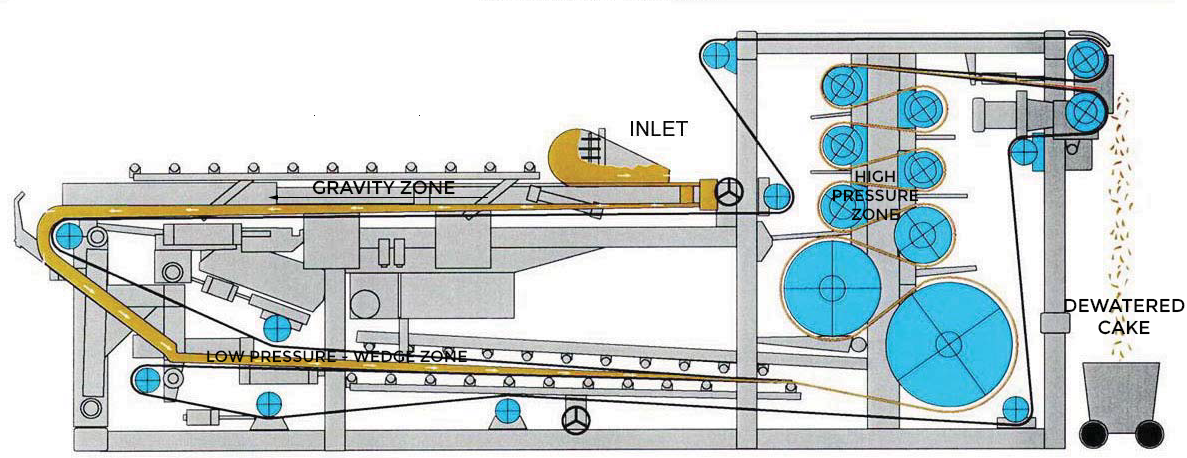
\includegraphics[scale=0.5]{BeltFilterPress}\\
		\vspace{1cm}
		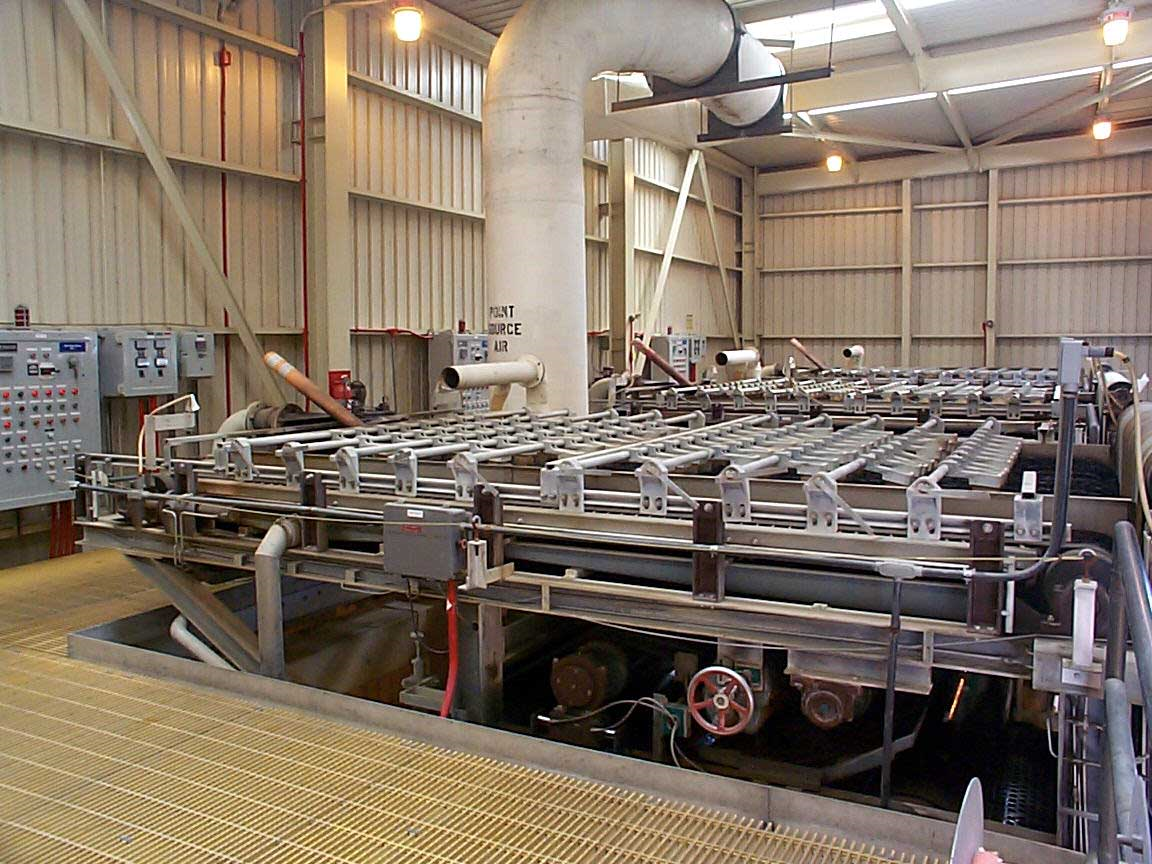
\includegraphics[scale=0.28]{BeltPressPicture}\\
		Belt Filter Press
		\end{center}

\subsection{Principles of belt filter press operations}\index{Principles of belt filter press operations}
					\begin{itemize}
						\item Belt filter press utilizes two endless, porous belts (generally 0.7 to 3 meter wide) made from a synthetic material
						\item Polymer flocculated sludge is first introduced on the horizontal \hl{gravity zone} of the press where free water is removed from the sludge by chicane assisted gravity filtration through the porous belt press fabric.
						\begin{center}
						\includegraphics[scale=0.2]{Chicanes}\\
						Gravity Zone - Chicanes
						\end{center}
						\item From the gravity zone, the sludge enters the \hl{low pressure zone (wedge zone)} in which the sludge is prepared for the upcoming \hl{high-pressure zone} by evenly distributing the solids across the belt and gradually applying pressure
						\item In the high pressure zone the sludge is sandwiched between two belt press fabrics. As the belts with the sandwiched sludge passes over and under 6 to 12 tensioning rollers which progressively decrease in diameter.  The applied pressure squeezes the water out from the sludge and is removed through the porous fabric.
						\item The filtrate is returned back to the front of the plant.
						\item The belts are washed continuously as they pass over \hl{wash boxes}.  The wash boxes are equipped with rotating brushes and water sprays and are primarily for keeping the belt press fabric pores open so water could easily filter through.  
						\item Improper polymer dosage and excessive hydraulic loading can lead to a wetter sludge cake.
						\item The belts are operated at speeds that commensurate with the rate of solids loading and the type of sludge being dewatered. Lower belt speed would allow for better water removal.  However, if if the belts speed is below the threshold for that particular sludge, belt press \hl{washout}, which is characterized by sludge flowing over the sides of the belt can occur .  Thus, the best belt speed is the slowest speed the belt can be operated without causing washout.
						\item The belts can be blinded - loose its porosity causing the water to stagnate/cause washout and not filter through, if excessive polymer is used or due ineffective belt washing.
						\item \hl{Solids capture rate} and \hl{Percent cake solids} produced are the most important belt press efficiency measurement parameters
					\end{itemize}
\subsection{Elements of the belt filter press}\index{Elements of the belt filter press}


 
						\begin{itemize}
							\item belts
							\item wash boxes
							\item guiding and tensioning rollers
							\item chicanes 
							\item doctor blades
							\item drive motor
							\item hydraulic unit
							\item polymer injection and mixing system
						\end{itemize}

\subsection{Belt press operational parameters}\index{Belt press operational parameters}


						\begin{itemize}
							\item belt filter width
							\item belt filter speed
							\item hydraulic loading
							\item belt tension
							\item washout
							\item filtrate quality
							\item solids capture rate
							\item polymer dosing rate (lbs polymer/dry ton solids)
							\item solids and hydraulic loading rates, and
							\item quantity and characteristics of the polymer used
						\end{itemize}

\section{Centrifuge}\index{Centrifuge}
			The centrifuge dewaters the sludge by subjecting a polymer conditioned sludge to strong centrifugal forces by rotating it in a bowl at high speeds.  Centrifuges are used for dewatering solids in many different applications and wastewater solids dewatering being one them.  Centrifuges also come in different configurations.  The scroll conveyor (decanter) centrifuge is the more commonly used centrifuge design for wastewater sludge dewatering.  It produces a dewatered product typically between 20\% to 30\% solids content.  It should be noted that the centrifuge can also be utilized for sludge thickening.

			\begin{center}
				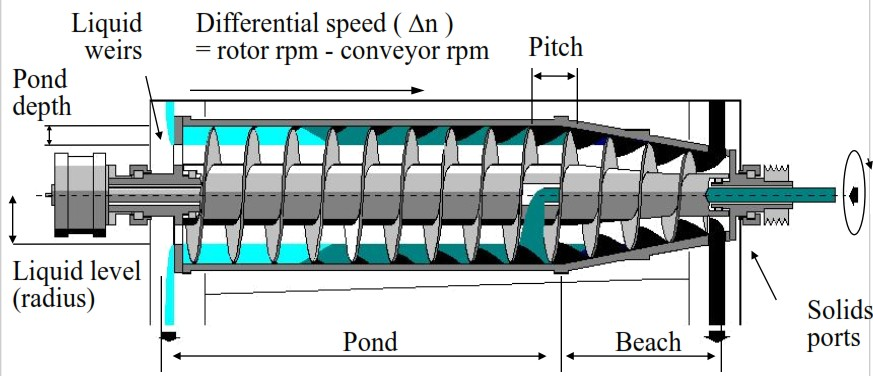
\includegraphics[scale=0.4]{Centrifuge3}\\
				Centrifuge
			\end{center}
\section{Principles of centrifuge operations}\index{Principles of centrifuge operations}
				\begin{itemize}
					\item The bowl of the centrifuge is cylindrical shaped with a tapered cone at one end.  The bowl is designed to rotate at speeds of 1200 to 2400 RPM.
						\begin{center}
							\includegraphics[scale=0.40]{Centrifugebowl}\\
							\vspace{1cm}
							\includegraphics[scale=0.2]{CentrifugebowlPicture}\\
							Centrifuge Bowl
						\end{center}
					\item A screw conveyor - scroll is shaped to the bowl  contour and carried on a central shaft or drum and it rotates independently from the bowl.  
						\begin{center}
							\includegraphics[scale=0.50]{Centrifugescroll}\\
							\vspace{1cm}
							\includegraphics[scale=0.2]{CentrifugescrollPicture}\\
							Centrifuge Scroll
						\end{center}
					\item The polymer conditioned sludge is fed into the cylindrical portion of the bowl through a central feed pipe.  Inside the bowl, the sludge is subjected to intense G forces around 3000 Gs by virtue of the bowl rotating at a high speed. 
					\item As the bowl rotates, the water in the flocculated sludge is separated from the solids .  
					\item The scroll rotates at a 5 to 15 rpm differential speed from the bowl.  This differential speed causes the thickened  sludge to be propelled  along the bowl for towards its conical end.  As the sludge is screwed up the cone it emerges from the liquid at the beach, is drained and pushed up to discharge ports.  
					\item The separated water is discharged from the cylindrical (non-conical) end of the bowl.  The depth of the water - \hl{pond depth}, is controlled by adjustable weirs at the discharge end.
					\item The greater the pond depth improves the centrate quality and solids recovery but it reduces the drainage zone at the \hl{beach} end resulting in wetter solids.  The pond depth is altered using adjustable weirs.
					\item The centrate is returned back to the front of the plant 
				\end{itemize}
	
\section{Elements of the Centrifuge}\index{Elements of the Centrifuge}	


					\begin{itemize}
						\item bowl
						\item scroll
						\item beach
						\item adjustable weir
						\item differential gear box
						\item drive motor
					\end{itemize}

\section{Centrifuge operational parameters}\index{Centrifuge operational parameters}	
					\begin{itemize}
						\item bowl speed
						\item differential speed
						\item pond height
						\item centrate quality
						\item solids capture rate
						\item polymer dosing rate (lbs polymer/dry ton solids)
						\item solids and hydraulic loading rates
					\end{itemize}

\section{Dewatering math problems}\index{Dewatering math problems}

\subsection{Calculation of solids recovery}\index{Calculation of solids recovery}



                \hl{Example Problems:}\\


(a) Calculate amount of solids fed to the dewatering unit\\
(b) Calculate the amount of solids produced as part of the dewatered cake\\
(c) The ratio of the solids in dewatered cake to that in the feed times 100 will give you the solids\\
recovery (solids recovery rate)\\


\subsection{Calculation of dewatered cake volume}\index{Calculation of dewatered cake volume}

(a) First calculate the amount of cake solids produced in terms of weight per time.\\
(b) From the weight of the cake produced calculate the volume - from the cake density which is
normally given\\

\subsection{Hauling cost impact due to solids content change}\index{Hauling cost impact due to solids content change}

(a) First calculate the amount of dry solids produced as part of the original wet cake solids percent\\
(b) Using the value of the dry solids calculate the wet cake weight with the new cake solids percentage\\

General formula for calculating net savings associated with change in cake solids content:\\
$Savings = \dfrac{(New \enspace solids(\%) - Old \enspace Solids(\%)}{New \enspace solids(\%)}*Old \enspace Cost$\\
So if the average cake dryness goes up from 20\% to 26\% and currently this utility is spending \$ 1,000,000 per
year for biosolids hauling and disposal, their net savings will be:\\
$\dfrac{(26\%-20\%)}{26\%}* 1,000,000 = \$230,769$\\
\hl{Example Problems}\\
\begin{enumerate}[1.]


\item 12,000 $ft^3$ of anaerobically digested sludge containing 2.8\% TS is dewatered in a centrifuge.  The centrifuge yields 37 $yd^3$ of 26\% of dewatered cake with a density of 73 lb/$ft^3$.  Calculate the solids capture rate.\\


 

Solution:\\
$
    lbs \enspace TS \enspace feed \enspace to \enspace centrifuge
    =
    12,000 ft^3 \enspace sludge
    *
    7.48 
    \dfrac
    {
    gal
    }
    {
    ft^3
    }
    *
    \dfrac
    {
    (8.34*0.028 lbs \enspace TS )
    }
    {gal \enspace sludge
    }
    =20,960 {lbs \enspace TS}
$

$
    lbs \enspace TS \enspace feed \enspace from \enspace centrifuge
    =
    37 yd^3 \enspace sludge
    *
    27 
    \dfrac
    {
    ft^3
    }
    {
    yd^3
    }
    *
    \dfrac
    {
    (73 lbs *0.26 \enspace TS )
    }
    {ft^3 \enspace sludge
    }
    =18,961 {lbs \enspace TS}
$

$
    solids \enspace capture \enspace rate
    =
    \dfrac
    {
    18,961 lbs \enspace solids \enspace produced        \enspace by \enspace centrifuge
    }
    {
    20,960 lbs \enspace solids \enspace fed             \enspace from \enspace digester
    }
    *
    100 
    =\boxed
    {
    90.4\% solids \enspace capture
    }
$


\item At a 60 GPM of 2.8\% feed a belt press which has a 90\% solids capture rate produces a 20\% cake at 68 lbs/$ft^3$.  How long would it take to fill a 3 $yd^3$ bin  
    
    
Solution:\\
{$\dfrac{cake \enspace TS \enspace produced - lbs}{min}= \dfrac {60 gallons \enspace sludge}{min}*\dfrac {8.34 lbs \enspace sludge \enspace feed}{galllon}*\dfrac{0.028 lbs \enspace TS}{lb \enspace sludge}*0.9$}\\
\vspace{3mm}

{$=\dfrac{12.61lbs \enspace TS}{min}$}\\
\vspace{3mm}

{$\dfrac{ft^3 \enspace cake \enspace produced}{min}=\dfrac{12.61lbs \enspace TS}{min}*\dfrac{100 lbs \enspace cake}{20lbs \enspace TS}*\dfrac{ft^3 \enspace cake}{68 lbs \enspace cake} = \dfrac{0.927ft^3 cake}{min}$}\\
\vspace{3mm}

{$\dfrac{ft^3 \enspace cake \enspace produced}{min}=\dfrac{12.61lbs \enspace TS}{min}*\dfrac{100 lbs \enspace cake}{20lbs \enspace TS}*\dfrac{ft^3 \enspace cake}{68 lbs \enspace cake} = \dfrac{0.927ft^3 cake}{min}$}\\
\vspace{3mm}

{$Time \enspace required \enspace to \enspace fill \enspace the \enspace bin=\dfrac{min}{0.927ft^3}*{3yd^3}*\dfrac{27ft^3}{yd^3}=\boxed{75min}$}\\


\end{enumerate}

